\documentclass{beamer}
\author{Joe Bentley and Jake Lane}
\usepackage{mathtools, amsmath, xcolor, graphicx}
\usetheme{Rochester}
\usecolortheme{dolphin}
\title{Higgs Signal optimisation}
\institute{}
\subject{Physics}
\date{}
\begin{document}
\frame{\titlepage}
\frame{
\frametitle{Summary}
\begin{enumerate}
\item General background on Higgs
\item How Higgs signals are simulated
\item How the Higgs signal is optimised
\item Problems in optimisation and improvements
\item Possible expansions of the project
\end{enumerate}
}
\frame{
\frametitle{Background}
The Higgs boson is produced in many channels.
\pause
The most common in proton collider experiments is 'gluon gluon Fusion' (ggF)
\begin{figure}
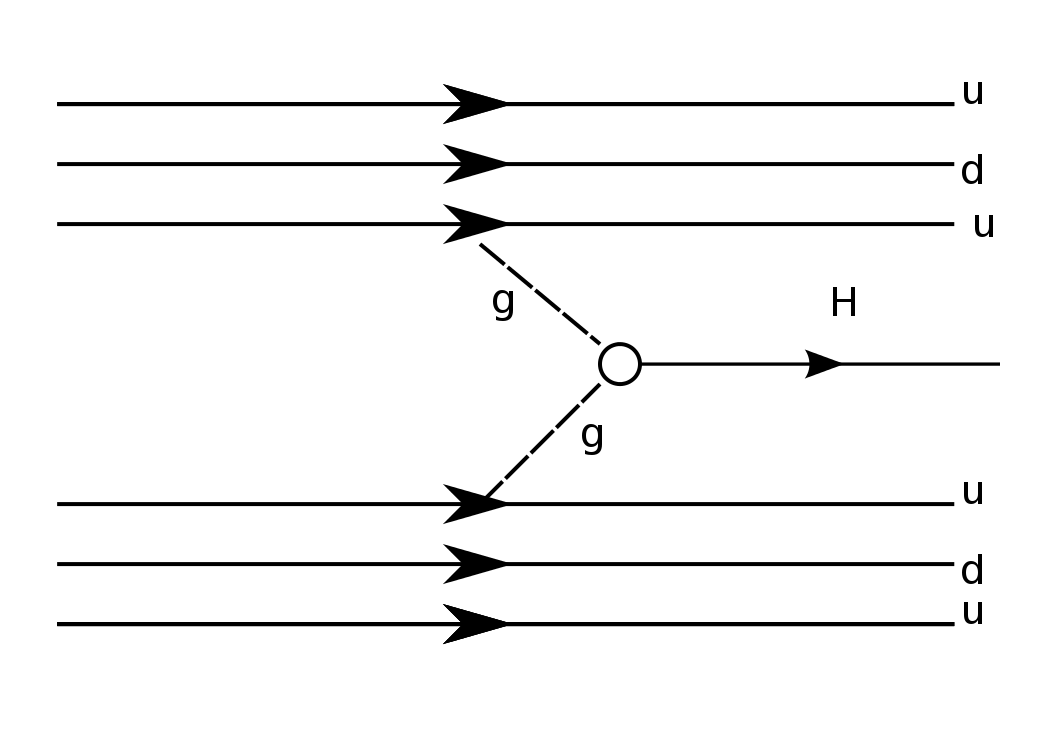
\includegraphics[scale = 0.2]{VBF.png}
\caption{Gluons fusing into a Higgs at a proton-proton interaction}
\end{figure}
\pause
The Higgs decays in a very short period of time in many channels, the most common is 2 bottom quarks, but we investigate the decay into 2 photons (the diphoton channel.)
}
\frame{
\begin{figure}
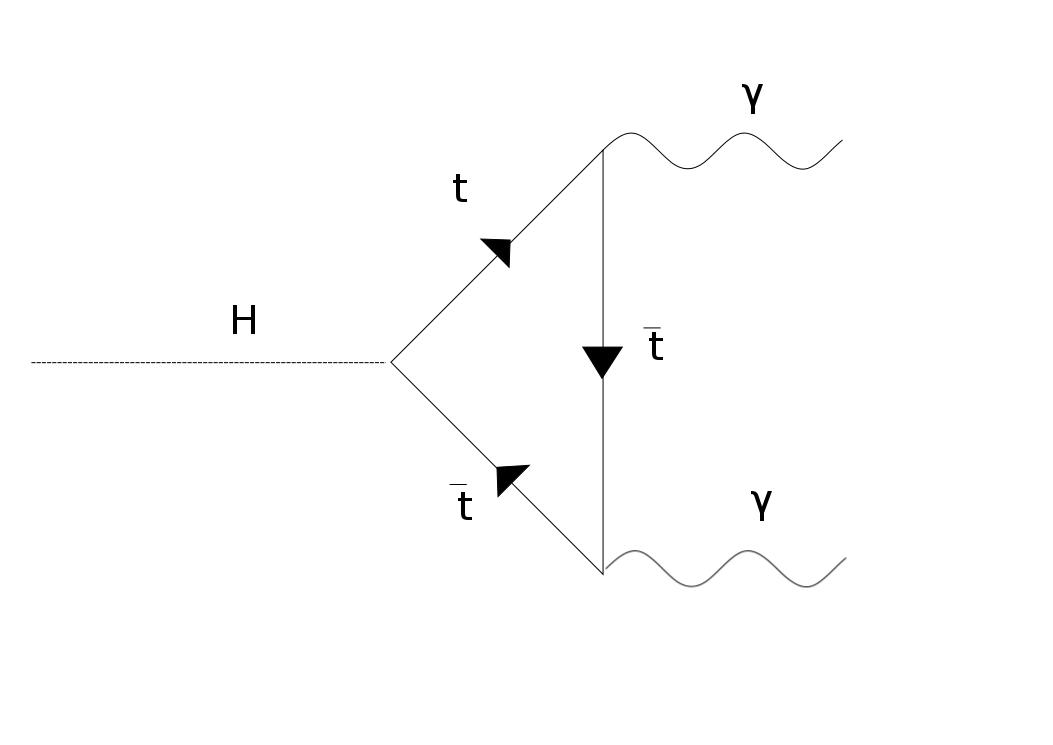
\includegraphics[scale=0.2]{Hyy.png}
\caption{Decay of Higgs into 2 photons}
\end{figure}
This has a branching fraction of order of  $10^{-3}$ but is much  easier to detect experimentally.
}
\frame{
\frametitle{Simulation}
The Higgs events and background events are simulated using PYTHIA. The simulation consists of a text file of the Energy and momentum (4 momentum) of each photon in each event (read collision.) We will use 1 simulation of Higgs events (which still have background in them) and 1 simulation of background events.


\pause


We need to filter out all of the combined events so that the statistical significance, $\Sigma$, is as high as possible.
\begin{equation}
\Sigma \equiv \frac{S}{\sqrt{S + B}}
\end{equation}

    
Where $S$ is the number of filtered signal (from the simulation) events and $B$ is the number of filtered background events (also simulated.)
}
\end{document}
